\subsection{Validazione e collaudo}
Periodo: dal \textbf{2022-03-20} al \textbf{2022-04-07} \mbox{} \\ \mbox{} \\
Le precondizioni sono:
\begin{itemize}
	\item le postcondizioni della fase precedente sono state soddisfatte.
\end{itemize} \mbox{} \\
Le postcondizioni sono:
\begin{itemize}
	\item aggiornamento ed approvazione dei documenti prodotti precedentemente;
	\item esecuzione di tutti i test;
	\item completamento del prodotto software;
	\item realizzazione della presentazione da esporre nella terza revisione: la \textit{Customer Acceptance}. 
\end{itemize} \mbox{} \\
La fase è composta da una nuova attività:
\begin{itemize}
	\item \textbf{Incremento e verifica dei documenti}: viene aggiornata e migliorata la documentazione;
	\item \textbf{Incremento e verifica delle attività}: se necessario, vengono migliorate le attività di \textit{Technology Baseline}, per quanto riguarda la progettazione ad alto livello, la \textit{Product Baseline}, riguardo l’aggiunta di design pattern o diagrammi delle classi e di attività, e la Codifica, formata seguendo l’idea di incrementi ciclici come per la fase precedente. In particolare, se non ci sono stati ritardi nella codifica si terrà in considerazione l’idea di implementare uno o più casi d’uso opzionali; di conseguenza, al momento non verranno pianificati gli incrementi in maniera esatta, poiché ritenuti troppo prematuri;
	\item \textbf{Validazione e collaudo}: realizzazione degli ultimi test con successivi controlli finali per verificare se le funzionalità soddisfano i risultati attesi secondo quanto indicato nel \textit{Piando di Qualifica}.
\end{itemize}

\subsubsection{Periodi}

Questa fase è stata suddivisa in tre periodi distinti, che andremo ad analizzare in seguito.

\subsubsubsection{I Periodo}

\textbf{dal 2022-03-20 al 2022-03-24}: in questo primo periodo il gruppo si dedicherà, se necessario, a migliorare con oppurtune correzioni i documenti prodotti precedentemente, inclusi quelli per la \textit{Technology Baseline} e \textit{Product Baseline}. Inoltre, si controllerà che i requisiti obbligatori siano soddisfatti.

\subsubsubsection{II Periodo}

\textbf{dal 2022-03-24 al 2022-04-01}: nel secondo periodo il team si dedicherà unicamente alla codifica e alla realizzazione dei test.

\subsubsubsection{III Periodo}

\textbf{dal 2022-04-01 al 2022-04-07}: nell'ultimo periodo, si incrementeranno i documenti di specifica tecnica e manuale utente, in base a quanto ulteriormente aggiunto nei periodi precedenti. Infine, si verificherà di aver realizzato tutti i test per la validazione ed il collaudo, oltre a produrre il materiale necessario da esporre in sede di presentazione del prodotto finale.

\begin{figure}[H]
\centering
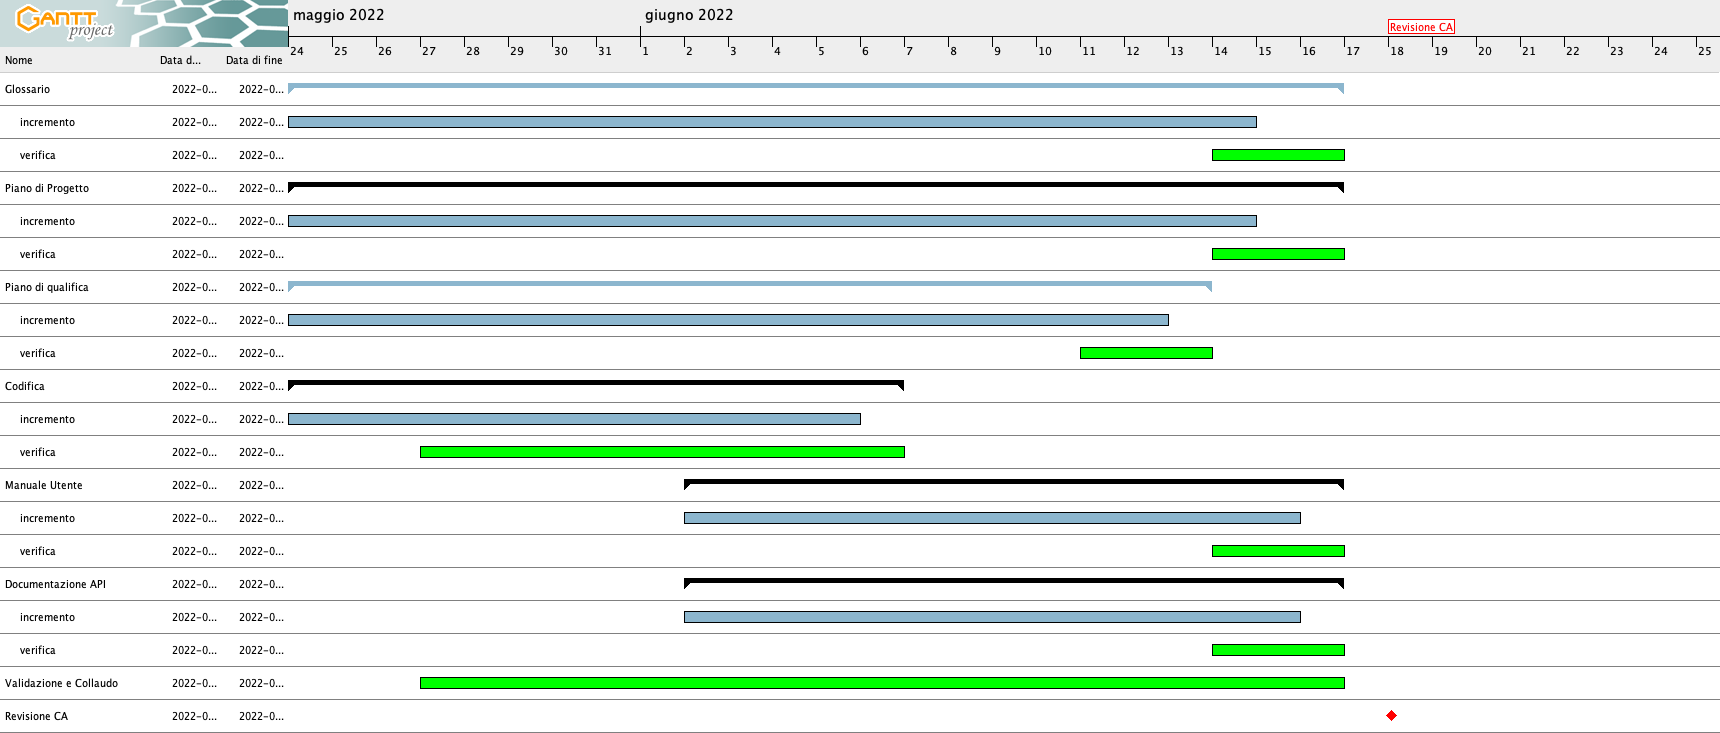
\includegraphics[scale=0.35]{Sezioni/gantt/validazione_collaudo.png}
\caption{Diagramma di Gantt - Validazione e collaudo}
\end{figure}